\chapter{MARCO TEORICO}
\section{Registros de eventos (logs)}
Los registros de eventos, comúnmente denominados \textit{logs}, son registros cronologicos generados por sistemas informáticos, aplicaciones, servidores y dispositivos de red como resultado de las diferentes actividades que se llevan a cabo durante su operación. Estos registros permiten conservar información sobre acontecimientos importantes del sistema, proporcionando evidencia sobre su funcionamiento, cambios de estado, errores y accesos.

La información contenida en un registro depende de la aplicación o dispositivo que lo genera. Sin embargo, generalmente un evento puede contener elementos como una marca temporal, la identificación del dispositivo o sistema que lo generó, el proceso o servicio asociado, un nivel de severidad y una descripción del acontecimiento. La combinación de estos elementos permite establecer el contexto en el que ocurrió un evento y facilita su posterior análisis.

\begin{lstlisting}[
    style=logstyle,
    caption={Ejemplo de un evento de cambio de estado de una interfaz},
    label={lst:log-cambio-estado},
    captionpos=b
]
Aug 12 10:35:22 router01 Interface ge-0/0/1 changed state to down
\end{lstlisting}

Sin embargo, los distintos fabricantes y aplicaciones pueden seguir formatos de registro propios a pesar de que existen estandares establecidos, por esta razon no es posible categorizar el origen de los registros de eventos de manera uniforme.
Afortunadamente, todos estos eventos pueden categorizarse por niveles de severidad, que van desde información general hasta errores críticos que requieren atención inmediata. La correcta gestión y análisis de los registros de eventos es fundamental para la administración de sistemas, la resolución de problemas, la auditoría de seguridad y el cumplimiento de normativas y regulaciones.

\section{Protocolo Syslog}
Syslog es un estándar para el envío de mensajes de registro en una red informática IP. Por syslog se conoce tanto al protocolo de red como a la aplicación o biblioteca que envía los mensajes de registro.

\subsection{Estructura de los mensajes}
El protocolo establece una estructura para representar información relacionada con un evento, permitiendo incluir elementos que facilitan su identificación y clasificación, como su nivel de prioridad, la fuente que lo genera, una marca temporal y el contenido del mensaje. De esta manera, Syslog proporciona un mecanismo común para el intercambio de información de registro entre diferentes componentes de un sistema.

Entre las especificaciones más relevantes se encuentran el formato tradicional descrito en RFC 3164 y el formato definido posteriormente en RFC 5424, los cuales presentan diferencias tanto en la organización como en el nivel de estructuración de sus campos.

\subsubsection{Priority (PRI)}
El campo PRI, abreviatura de \textit{Priority}, es un elemento fundamental en la estructura de los mensajes Syslog, ya que representa la prioridad asignada a un mensaje y permite identificar tanto la categoría de origen del evento como su nivel de severidad. Este campo se encuentra al inicio del mensaje y se representa mediante un valor numérico encerrado entre los caracteres < y >.

El valor contenido dentro de PRI se obtiene mediante la combinación de dos componentes: Facility y Severity. El cálculo está definido mediante la expresión:

\begin{equation}
    PRI = (Facility \times 8) + Severity
\end{equation}

donde Facility identifica la categoría o subsistema que generó el mensaje, mientras que Severity representa la importancia o gravedad del evento.

\subsubsection{Facility}
El campo Facility permite clasificar el origen lógico del mensaje. Cada valor de Facility corresponde a un subsistema o componente específico del sistema que genera el evento:

\begin{longtable}{p{2.0cm} p{4.0cm} p{9.0cm}}
    \caption{Valores de Facility en Syslog}
    \label{tab:syslog_facility} \\

    \toprule
    \textbf{Valor} & \textbf{Facility} & \textbf{Descripción} \\
    \midrule
    \endfirsthead

    \multicolumn{3}{c}{\textit{Tabla \thetable. Continuación}} \\
    \toprule
    \textbf{Valor} & \textbf{Facility} & \textbf{Descripción} \\
    \midrule
    \endhead

    \midrule
    \multicolumn{3}{r}{\textit{Continúa en la siguiente página}} \\
    \endfoot

    \bottomrule
    \endlastfoot

    0 & \texttt{kern} &
    Mensajes generados por el kernel del sistema. \\

    1 & \texttt{user} &
    Mensajes generados por procesos o aplicaciones a nivel de usuario. \\

    2 & \texttt{mail} &
    Mensajes relacionados con el sistema de correo. \\

    3 & \texttt{daemon} &
    Mensajes generados por procesos del sistema ejecutados como demonios. \\

    4 & \texttt{auth} &
    Mensajes relacionados con procesos de autenticación. \\

    5 & \texttt{syslog} &
    Mensajes generados internamente por el propio sistema Syslog. \\

    6 & \texttt{lpr} &
    Mensajes relacionados con el sistema de impresión. \\

    7 & \texttt{news} &
    Mensajes relacionados con el sistema de noticias de red. \\

    8 & \texttt{uucp} &
    Mensajes relacionados con el protocolo UUCP. \\

    9 & \texttt{cron} &
    Mensajes relacionados con procesos de planificación de tareas. \\

    10 & \texttt{authpriv} &
    Mensajes relacionados con autenticación que contienen información privada. \\

    11 & \texttt{ftp} &
    Mensajes relacionados con el servicio FTP. \\

    12 & \texttt{ntp} &
    Mensajes relacionados con el protocolo NTP. \\

    13 & \texttt{security} &
    Mensajes relacionados con auditoría y seguridad. \\

    14 & \texttt{console} &
    Mensajes asociados con el uso de la consola. \\

    15 & \texttt{solaris-cron} &
    Mensajes relacionados con el planificador de tareas de Solaris. \\

    16 -- 23 & \texttt{local0 - local7} &
     Facilities reservadas para uso local y aplicaciones específicas. \\
\end{longtable}

\subsubsection{Severity}
El campo Severity, también conocido como nivel de severidad, indica la importancia o gravedad del evento registrado. Este campo permite a los administradores y sistemas de monitoreo priorizar la atención a los eventos según su criticidad, facilitando la identificación de problemas que requieren intervención inmediata frente a aquellos que son meramente informativos o de menor relevancia.

\begin{longtable}{p{2.0cm} p{4.0cm} p{9.0cm}}
    \caption{Niveles de Severity en Syslog}
    \label{tab:syslog_severity} \\

    \toprule
    \textbf{Valor} & \textbf{Severity} & \textbf{Descripción} \\
    \midrule
    \endfirsthead

    \multicolumn{3}{c}{\textit{Tabla \thetable. Continuación}} \\
    \toprule
    \textbf{Valor} & \textbf{Severity} & \textbf{Descripción} \\
    \midrule
    \endhead

    \midrule
    \multicolumn{3}{r}{\textit{Continúa en la siguiente página}} \\
    \endfoot

    \bottomrule
    \endlastfoot

    0 & \texttt{Emergency} &
    El sistema no puede utilizarse. Representa el nivel de mayor severidad. \\

    1 & \texttt{Alert} &
    Se requiere una acción inmediata para corregir la condición presentada. \\

    2 & \texttt{Critical} &
    Condición crítica que requiere atención inmediata y puede comprometer el funcionamiento del sistema. \\

    3 & \texttt{Error} &
    Se ha producido una condición de error que afecta el funcionamiento de un componente. \\

    4 & \texttt{Warning} &
    Se presenta una condición de advertencia que puede requerir atención. \\

    5 & \texttt{Notice} &
    Evento normal pero significativo que merece ser registrado. \\

    6 & \texttt{Informational} &
    Mensaje informativo sobre el funcionamiento o estado del sistema. \\

    7 & \texttt{Debug} &
    Información detallada utilizada principalmente para depuración y diagnóstico.

\end{longtable}

\subsubsection{RFC 3164}
El documento RFC 3164, denominado The BSD Syslog Protocol, publicado en 2001 por el IETF, describe una especificación para el formato de mensajes, basada en la implementación tradicional utilizada en sistemas BSD \cite{rfc3164}.

Utiliza un formato básico con codificación ASCII, no incluye año ni zona horaria en las marcas de tiempo y tiene un límite de 1024 bytes por mensaje. Ideal para sistemas heredados o configuraciones pequeñas.

La estructura de un mensaje RFC 3164 puede representarse conceptualmente como:

\begin{figure}[H]
    \centering
    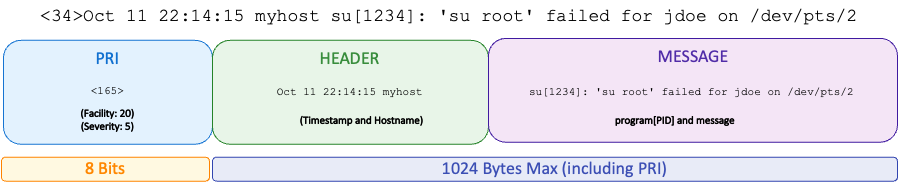
\includegraphics[width=0.8\textwidth]{Figuras/rfc3164.png}
    \caption{Estructura de un mensaje RFC 3164}
    \label{fig:rfc3164}
\end{figure}

La siguiente tabla describe los campos que componen un mensaje Syslog bajo este estandar.

\begin{longtable}{p{3cm} p{3cm} p{10cm}}
    \caption{Campos de un mensaje Syslog según RFC 3164}
    \label{tab:campos-rfc3164} \\

    \toprule
    \textbf{Campo} & \textbf{Valor} & \textbf{Descripción} \\
    \midrule
    \endfirsthead

    \multicolumn{3}{c}{\textit{Tabla \thetable. Continuación}} \\
    \toprule
    \textbf{Campo} & \textbf{Valor} & \textbf{Descripción} \\
    \midrule
    \endhead

    \midrule
    \multicolumn{3}{r}{\textit{Continúa en la siguiente página}} \\
    \endfoot

    \bottomrule
    \endlastfoot

    \texttt{PRI} &
    \texttt{<34>} &
    Indica la prioridad del mensaje y está compuesto por los valores de Facility y Severity. \\

    \texttt{TIMESTAMP} &
    \texttt{Oct 11 22:14:15} &
    Indica la fecha y hora en que se generó el evento. Utiliza el formato de mes, día, hora, minutos y segundos. \\

    \texttt{HOSTNAME} &
    \texttt{myhost} &
    Identifica el sistema o dispositivo que originó el mensaje. \\

    \texttt{TAG} &
    \texttt{su} &
    Permite identificar la aplicación o proceso asociado con la generación del mensaje. \\

    \texttt{PID} &
    \texttt{[1234]} &
    Identifica el proceso que generó el evento cuando el sistema emisor proporciona esta información. \\

    \texttt{MSG} &
    \texttt{'su root' failed for jdoe on /dev/pts/2} &
    Contiene la información específica del evento generado por la aplicación o dispositivo. \\

\end{longtable}

Una característica importante de RFC 3164 es que no define un esquema rígido para el contenido del campo MSG. El significado y formato de esta parte depende de la aplicación o dispositivo que genera el evento. Esto permite una gran flexibilidad, pero también introduce variabilidad entre fabricantes y sistemas.

A nivel de transporte, RFC 3164 contempla principalmente el uso de UDP, particularmente sobre el puerto 514, sin establecer mecanismos propios de confirmación, retransmisión o control de congestión. Por esta razón, el transporte definido bajo este modelo es de naturaleza no orientada a conexión y no garantiza la entrega de los mensajes.

Su diseño sencillo puede presentar dificultades en los entornos informáticos modernos. Por ejemplo, su formato de marca de tiempo carece de año y zona horaria, lo que puede generar confusión al correlacionar registros entre sistemas o durante investigaciones que abarcan varios periodos de tiempo. Actualente este estandar esta considerado como obsoleto y fue reemplazado formalmente por el estándar más completo RFC 5424, aunque sigue activo en algunos equipos y redes pequeñas.

\subsubsection{RFC 5424}
El RFC 5424, denominado The Syslog Protocol, fue publicado por el IETF en marzo de 2009, define un formato estandarizado para los mensajes del protocolo syslog \cite{rfc5424}. Su principal objetivo es proporcionar una estructura más precisa y extensible que la definida previamente por RFC 3164, algunas de las mejoras introducidas que buscan abordar las limitaciones son las siguientes:

\begin{itemize}
    \item RFC 5424 mejora considerablemente la representación temporal de los mensajes al incluir el año, la zona horaria y la posibilidad de registrar fracciones de segundo. Esto permite una mayor precisión en la marca temporal y facilita la correlación de eventos entre sistemas distribuidos.
    \item Introduce el campo STRUCTURED-DATA, lo que permite incorporar información estructurada dentro del mensaje. Esto hace posible que información que antes tendría que estar embebida en texto libre pueda representarse explícitamente como atributos.
    \item RFC 5424 utiliza $"-"$ como NILVALUE, es decir, indica que un determinado campo no tiene valor disponible. Esto facilita la interpretación de los mensajes y permite una mayor consistencia en la representación de datos faltantes.
\end{itemize}


La estructura de un mensaje RFC 5424 puede representarse conceptualmente como:

\begin{figure}[H]
    \centering
    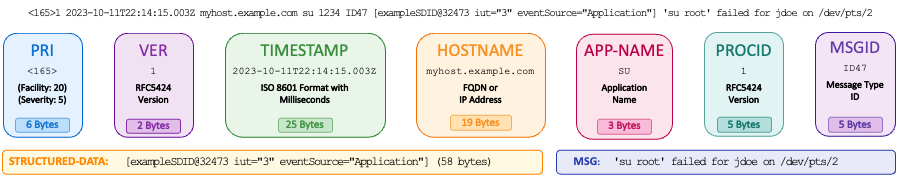
\includegraphics[width=1\textwidth]{Figuras/rfc5424.png}
    \caption{Estructura de un mensaje RFC 5424}
    \label{fig:rfc5424}
\end{figure}

La siguiente tabla describe los campos que componen un mensaje Syslog bajo este estandar.

\small
\begin{longtable}{p{3.0cm} p{2.0cm} p{10cm}}
    \caption{Campos del formato de mensaje Syslog definido en RFC 5424}
    \label{tab:rfc5424_fields} \\

    \toprule
    \textbf{Campo} & \textbf{Longitud} & \textbf{Descripción} \\
    \midrule
    \endfirsthead

    \multicolumn{3}{c}{\textit{Tabla \thetable. Continuación}} \\
    \toprule
    \textbf{Campo} & \textbf{Longitud} & \textbf{Descripción} \\
    \midrule
    \endhead

    \midrule
    \multicolumn{3}{r}{\textit{Continúa en la siguiente página}} \\
    \endfoot

    \bottomrule
    \endlastfoot

    \texttt{PRI} &
    1--3 caracteres &
    Contiene la prioridad del mensaje, calculada a partir de los valores de
    \textit{Facility} y \textit{Severity}. Se representa mediante un valor
    numérico encerrado entre los caracteres ``\texttt{<}'' y ``\texttt{>}''. \\

    \texttt{VERSION} &
    1--3 caracteres &
    Indica la versión del formato de mensaje Syslog utilizado. Para RFC 5424,
    el valor definido actualmente es \texttt{1}. \\

    \texttt{TIMESTAMP} &
    Variable &
    Indica la fecha y hora en la que se generó el evento. Utiliza un formato
    basado en ISO 8601 e incluye información de zona horaria y,
    opcionalmente, fracciones de segundo. \\

    \texttt{HOSTNAME} &
    Variable &
    Identifica el dispositivo o sistema que originó el mensaje. Puede
    corresponder al nombre de host, nombre de dominio o dirección IP del
    emisor, dependiendo de la información disponible. \\

    \texttt{APP-NAME} &
    1--48 caracteres &
    Identifica la aplicación o proceso que originó el mensaje. Permite asociar
    el evento con un componente específico del sistema emisor. \\

    \texttt{PROCID} &
    1--128 caracteres &
    Identifica el proceso que generó el mensaje. En sistemas donde sea
    aplicable, puede corresponder al identificador de proceso (PID). \\

    \texttt{MSGID} &
    1--32 caracteres &
    Identifica de forma única el tipo o clase de mensaje dentro del contexto
    de la aplicación que lo genera. Facilita la clasificación y correlación
    de eventos. \\

    \texttt{STRUCTURED-DATA} &
    Variable &
    Contiene información estructurada asociada al evento. Está formada por
    uno o más elementos de datos estructurados que pueden incluir parámetros
    con nombre y valor, facilitando el procesamiento automático de los
    mensajes. \\

    \texttt{MSG} &
    Variable &
    Contiene el contenido específico del evento. Puede incluir información
    adicional generada por la aplicación y, a diferencia de
    \textit{STRUCTURED-DATA}, generalmente se presenta como texto libre.

\end{longtable}

En cuanto a la longitud de los mensajes RFC 5424 no establece un límite máximo universal, el límite depende del transporte utilizado. Sin embargo, cualquier receptor debe poder aceptar mensajes de al menos 480 bytes y se recomienda que pueda aceptar hasta 2048 bytes.

Esto es relevante al trabajar con equipos de red porque algunos fabricantes generan mensajes considerablemente largos, especialmente cuando incluyen información estructurada o detalles adicionales del evento.

Finalmente, RFC 5424 define un mecanismo de transporte más flexible y confiable, permitiendo el uso de protocolos orientados a conexión como TCP y TLS, además del tradicional UDP. Estas especificaciones estan descritas en el RFC 5425 (TLS) \cite{rfc5425} y RFC 5426 (TCP) \cite{rfc5426}.

\section{Syslog-ng}
Syslog-ng es una aplicación de gestión de registros diseñada para la recopilación, procesamiento y distribución centralizada de mensajes de log. Su arquitectura permite recibir información proveniente de diferentes fuentes, aplicar operaciones de filtrado, análisis y transformación, y posteriormente enviar los mensajes procesados hacia uno o varios destinos.

Una de las principales características es su capacidad para trabajar con una gran variedad de fuentes y destinos. El proyecto soporta mecanismos de entrada y salida asociados con Syslog, texto no estructurado, colas de mensajes, bases de datos SQL y NoSQL y plataformas de procesamiento de grandes volúmenes de información. También dispone de integraciones con tecnologías como Elasticsearch, Apache Kafka y Hadoop.

La Open Source Edition (OSE) de syslog-ng es un proyecto de código abierto cuyo código fuente se encuentra disponible públicamente. El proyecto utiliza las licencias GNU General Public License (GPL) y GNU Lesser General Public License (LGPL), dependiendo del componente. La comunidad mantiene el código, documentación, correcciones y nuevas funcionalidades mediante un modelo de desarrollo abierto \cite{syslogng_community}.

\subsection{Arquitectura y procesamiento}
El funcionamiento de syslog-ng se basa en varios objetos de configuración que definen cómo deben ser recibidos y procesados los mensajes. Los principales componentes son sources, destinations, filters, parsers, rewrite rules, templates y log paths \cite{syslogng_documentation}.
\begin{equation}
\boxed{
\substack{\text{Fuente de}\\\text{eventos}}
\rightarrow
\substack{\text{SOURCE}\\\text{Recepción}}
\rightarrow
\substack{\text{FILTER / PARSER}\\\text{Clasificación y extracción}}
\rightarrow
\substack{\text{REWRITE}\\\text{Normalización}}
\rightarrow
\substack{\text{TEMPLATE}\\\text{Formateo}}
\rightarrow
\substack{\text{DESTINATION}\\\text{Entrega}}
}
\label{eq:flujo-syslog-ng}
\end{equation}

El funcionamiento de cada uno es el siguiente:

\subsubsection{Sources}
Representan los puntos de entrada de los mensajes
hacia syslog-ng. Mediante este componente se define el mecanismo utilizado para recibir los registros generados por dispositivos, aplicaciones o sistemas externos.

Entre las fuentes disponibles se encuentran los archivos locales, los
sockets del sistema y las conexiones de red mediante protocolos como UDP y TCP.

Un ejemplo de una fuente de red que recibe mensajes mediante UDP en el
puerto 514 es:

\begin{lstlisting}[style=logstyle]
source s_network {
    network(
        ip(0.0.0.0)
        port(514)
        transport("udp")
    );
};
\end{lstlisting}

En este caso, \texttt{s\_network} identifica la fuente y el controlador
\texttt{network} establece las características de la recepción de los
mensajes.

\subsubsection{Filters}
Los filtros permiten seleccionar los mensajes que cumplen
determinadas condiciones. Estas condiciones pueden estar relacionadas con campos del mensaje Syslog, como facility, severity, host de origen, aplicación o contenido del mensaje.

Por ejemplo, es posible crear un filtro para seleccionar únicamente mensajes relacionados con autenticación:

\begin{lstlisting}[style=logstyle]
filter f_auth {
    facility(auth);
};
\end{lstlisting}

Los filtros pueden combinarse mediante operadores lógicos para construir condiciones más específicas. Esto permite separar los eventos según su naturaleza antes de enviarlos hacia los destinos correspondientes.

\subsubsection{Parsers}
Permiten analizar el contenido de los mensajes y
extraer información estructurada. Esta funcionalidad es especialmente importante cuando los dispositivos utilizan formatos propios o cuando la información relevante se encuentra dentro del campo de mensaje como por ejemplo:

\begin{lstlisting}[style=logstyle]
user=jdoe src=192.168.1.25 action=login status=failed
\end{lstlisting}

puede ser procesado para obtener diferentes campos:

\begin{lstlisting}[style=logstyle]
user   = jdoe
src    = 192.168.1.25
action = login
status = failed
\end{lstlisting}

Luego la informacion extraida se usa con mayor facilidad en filtros, reescrituras y plantillas.

\subsubsection{Rewrite}

Permiten modificar los valores asociados a un mensaje durante su procesamiento. Pueden utilizarse para reemplazar,
eliminar o establecer valores con el objetivo de normalizar la información proveniente de diferentes fuentes, como por ejemplo cuando diferentes dispositivos representan un mismo evento mediante expresiones diferentes:

\begin{lstlisting}[style=logstyle]
Login failed
Authentication failure
AUTH_FAIL
\end{lstlisting}

Mediante reglas de reescritura, estos valores pueden transformarse en una representación común:

\begin{lstlisting}[style=logstyle]
event_type=authentication_failure
\end{lstlisting}

Esta capacidad es muy fuerte en infraestructuras heterogéneas, ya que permite establecer una representación uniforme antes de entregar los eventos a una plataforma de análisis.

\subsubsection{Templates}
Definen la representación final de los mensajes
que serán enviados a un destino. Estas utilizan macros y valores estructurados disponibles durante el procesamiento para construir el contenido de salida.

Por ejemplo, puede definirse una plantilla para generar una estructura JSON:

\begin{lstlisting}[style=logstyle]
template t_json {
    template("{\"host\":\"${HOST}\",
\"program\":\"${PROGRAM}\",
\"message\":\"${MESSAGE}\"}\n");
};
\end{lstlisting}

Las plantillas permiten adaptar el formato de los registros a los requerimientos del sistema que los recibe.

\subsubsection{Destinations}

Representan los puntos hacia los cuales syslog-ng entrega los mensajes después de su procesamiento. Un destino puede corresponder a un archivo local, una base de datos, un servicio remoto o un dispositivo externo.

Por ejemplo, para almacenar los mensajes en un archivo:

\begin{lstlisting}[style=logstyle]
destination d_logs {
    file("/var/log/network.log");
};
\end{lstlisting}

Y para configurarse un destino de red para reenviar los mensajes hacia otro servidor:

\begin{lstlisting}[style=logstyle]
destination d_wazuh {
    network(
        "192.168.1.100"
        port(514)
        transport("udp")
    );
};
\end{lstlisting}

En la arquitectura implementada en el proyecto, este mecanismo permite utilizar syslog-ng como intermediario entre los dispositivos que generan los registros y la plataforma Wazuh.

\subsubsection{Log paths}
Definen las rutas de procesamiento que siguen los mensajes dentro de syslog-ng. En ellos se relacionan las fuentes, filtros, procesadores y destinos, estableciendo de esta manera el flujo de los registros:

\begin{lstlisting}[style=logstyle]
log {
    source(s_network);
    filter(f_auth);
    destination(d_wazuh);
};
\end{lstlisting}

En este caso, los mensajes recibidos mediante \texttt{s\_network} son evaluados por el filtro \texttt{f\_auth}. Aquellos que cumplen la condición establecida son enviados posteriormente hacia \texttt{d\_wazuh}.

Los log paths constituyen, por tanto, el mecanismo mediante el cual los diferentes componentes de syslog-ng se integran para construir el flujo de procesamiento de los registros.

\section{Sistemas de Gestión de Información y Eventos de Seguridad (SIEM)}
\section{Wazuh}
\section{Correlación de eventos}
\section{Detección y respuesta ante incidentes}